\title{19. Průběh funkce}
\author{Jakub Sláma}
\date{26.4.2025}

\maketitle

\section{Průběh funkce}
Vyšetřování průběhu funkce má několik kroků, následuje jejich seznam a popis:
\begin{enumerate}
    \item 
        \begin{itemize}
            \item Definiční obor 
            \item sudost nebo lichost
            \item periodičnost
        \end{itemize}
    \item
        \begin{itemize}
            \item jednostranné limity v bodech, kde není funkce definována
            \item limity v nevlastních bodech
        \end{itemize}
    \item
        \begin{itemize}
            \item průsečíky s osami x a y
            \item znaménka funkčních hodnot
        \end{itemize}
    \item
        \begin{itemize}
            \item první derivace, první derivace rovna 0, kde není definována
            \item intervaly monotónnosti, stacionární body
        \end{itemize}
    \item
        \begin{itemize}
            \item druhá derivace, druhá derivace rovna 0, kde není definována
            \item intervaly konvexnosti (nad tečnou) a konkávnosti (pod tečnou), extrémy, inflexní body
        \end{itemize}
    \item
        \begin{itemize}
            \item asymptoty bez směrnice $x=a$
            \item asymptoty se směrnicí $y=ax+b$
        \end{itemize}
    \item
        \begin{itemize}
            \item graf funkce
            \item obor hodnot
        \end{itemize}
\end{enumerate}

Vyšetřujeme funkci: 
$$
    f: y=\frac{x}{x^2+1}
$$
\subsection{Definiční obor, sudost nebo lichost, periodičnost}
\subsubsection{Obor hodnot}
Obor hodnot získáme zjištěním hodnot, které mohou být dosazeny za $x$.
V našem případě $D(f) \in R$
\subsubsection{Zjištění sudosti}
Funkce $f(x)$ je sudá, pokud platí:
$$
    f(-x)=f(x)
$$
(pokud se skládá z sudých funkcí a konstant) \\
Typickými sudími funkcemi je funkce kvadratická, nebo kubická.
\subsubsection{Zjištění lichosti}
Funkce $f(x)$ je lichá, pokud platí:
$$
    f(-x)=-f(x)
$$
(pokud se skládá z lichých funkcí a konstant)\\
\subsubsection{Periodičnost}
Funkce je periodická za předpokladu, že její průběh periodicky opakuje. Zástupci jsou například: $\sin(x); \cos(x); \tan(x); \cot(x)$
\subsubsection{Výpočet}
v našem případě:
$$
    f(-x)=\frac{-x}{(-x)^2+1}
$$

$$
    -\frac{x}{x^2+1}=\frac{-x}{(-x)^2+1}
$$
$$
    f(-x)=-f(x)
$$
při porovnání funkce po úpravách zjistíme, že je funkce lichá
\subsection{Limity vlastní a nevlastní}
Je nutno spočítat limity ve všech krajních bodech těch intervalů, které tvoří
definiční obor funkce $f$, pokud v nich tato funkce není přímo definovaná. Tj. jde většinou o jednostranné limity. Speciálně půjde často o limity v $+\infty; -\infty$
\\ \\
Např. v intervalech $(-\infty; 0)(0; \infty)$ rovnice $y=\frac{1}{x}$
$$
    \lim_{x\rightarrow0}{\frac{1}{x}}=0
$$
+ limity jdoucí do +, - nekonečna
\subsubsection{Jednostranné limity v bodech, kde není funkce definována}
Jednostranná limita je v infinitezimálním počtu libovolná z limit funkce $f(x)$ reálné proměnné $x$, u nichž se $x$ přibližuje k zadanému bodu buď zleva nebo zprava
\subsubsection{Limity v nevlastních bodech}
Limity v nevlastních bodech se týkají situací, kdy proměnná 
$x$ směřuje k nekonečnu nebo minus nekonečnu.
\subsubsection{Výpočet}
u této funkce $D(f) \in \mathbb{R}$, tudíž počítáme pouze limity jdoucí do +, - nekonečna  

$$
    \lim_{x\rightarrow\infty}{\frac{x}{x^2+1}}=0
$$
$$
    \lim_{x\rightarrow-\infty}{\frac{x}{x^2+1}}=0
$$

Tato funkce se blíží z obou stran k nule .
\subsection{Průsečíky s osami $x$ a $y$, znaménka funkčních hodnot}
\subsubsection{Průsečíky s osami $x$ a $y$}
Průsečíky s osami hodnot získáme dosazením 0 nejprve za $x$ souřadnici, poté za $y$
\subsubsection{Znaménka funkčních hodnot}
Za pomocí nulových bodů si vytvoříme tabulku, ve které zjistíme v kterých intervalech je funkce kladná a v kterých je záporná
\subsubsection{Výpočet}
1. výpočet průsečíku s osou $x$ ($y=0$)
$$
    0=\frac{x}{x^2+1}
$$
$$
    0=x
$$
souřadnice průsečíku funkce s osou x je $X[0;0]$ \\
2. výpočet průsečíku s osou $y$ ($x=0$)
$$
    y=\frac{0}{0^2+1}
$$
$$
    y=0
$$
souřadnice průsečíku funkce s osou y je $Y[0;0]$

$$
\begin{array}{|c|c|c|c|}
\hline
\textbf  & (-\infty;0\rangle & (0; \infty) \\
\hline
x     & - & + \\
x^2+1 & + & + \\
\hline
 & - & + \\
\hline
\end{array}
$$
Funkce v intervalu nabývá záporné hodnoty $(-\infty;0\rangle$ a v intervalu $(0; \infty)$ nabývá kladné hodnoty.

\subsection{První derivace, první derivace rovna 0, kde není definována, intervaly monotónnosti, stacionární body}
\subsubsection{První derivace, první derivace rovna 0, kde není definována}
První derivací zjistíme v kterých intervalech je funkce rostoucí, nebo klesající\\ \\
Pokud položíme první derivaci funkce rovnou nule body podezřelé z lokálních minim a maxim. \\ \\
Derivace také nemusí být definovaná, pokud má v nějakém bodě: \\
1. Nevlastní limitu (např. asymptotu) \\ 
2. Ostrý zlom (např. absolutní hodnota $y=|x|$ v bodě $x=0$)

\subsubsection{Intervaly monotónnosti, stacionární body}
Interval monotónnosti je část definičního oboru funkce, kde funkce buď stále roste, nebo stále klesá\\ \\
Stacionární bod je bod na grafu funkce, kde je první derivace rovna nule: $f'(x) = 0$ Funkce v tomto bodě může mít extrém (maximum, minimum)

\subsubsection{Výpočet}
nejprve zderivujeme výraz
$$
    f: y=\frac{x}{x^2+1} 
$$\\
$$
    y'=\frac{1(x^2+1)-x(2x)}{(x^2+1)^2}= \frac{x^2+1-2x^2}{(x^2+1)^2}=\frac{-x^2+1}{(x^2+1)^2}
$$\\
Následně výraz dáme roven 0, tímto zjistíme stacionární body
$$
    \frac{-x^2+1}{(x^2+1)^2} = 0
$$
Jsou dva $[1;0];[-1;0]$, následně zjistíme v kterých intervalech je funkce rostoucí a v kterých klesající:
$$
\begin{array}{|c|c|c|c|}
\hline
\textbf  & (-\infty;-1\rangle&(-1;1) & \langle 1; \infty) \\
\hline
-x^2+1  &   -  & + & - \\
(x^2+1)^2  & + & + & +\\
\hline
 & - & + & - \\
\hline
\end{array}
$$
Z tohoto vylívá, že funkce je klesající v intervalech $(-\infty;-1\rangle \cup \langle 1; \infty)$ klesající a v intervalu $(-1;1)$ rostoucí. \\ \\
Musíme dosadit body monotónnosti do původní rovnice, aby jsme získali souřadnice minim a maxim.
$$
    f: y=\frac{x}{x^2+1} 
$$\\
pro $x = 1$
$$
    f: y=\frac{1}{1^2+1} =\frac{1}{2}
$$
Souřadnice maxima je $[1;\frac{1}{2}]$
pro $x = -1$
$$
    f: y=\frac{-1}{(-1)^2+1} =-\frac{1}{2}
$$
Souřadnice minima je $[1;-\frac{1}{2}]$

Minimum je mezi klesajícím a rostoucím intervalem. \\
Maximum je mezi rostoucím a klesajícím.

\subsection{Druhá derivace, druhá derivace rovna 0, kde není definována, intervaly konvexnosti (nad tečnou) a konkávnosti (pod tečnou), inflexní body}

\subsubsection{Druhá derivace, druhá derivace rovna 0, kde není definována,}
Pomocí druhé derivace zjistíme tvar křivky (konkávnost, konvexnost) za pomocí intervalů (v kladných je funkce konvexní (nad tečnou $\cup$), v záporných je konkávní (pod tečnou $\cap$))  \\
Druhou derivaci funkce pokládáme nule, aby jsme zjistily inflexní body (body, ve kterých se mění zakřivení grafu funkce) \\
druhá derivace není definována, pokud:
\begin{itemize}
    \item Funkce není dostatečně hladká – není spojitá nebo není dostatečně "plynulá"
    \item První derivace není spojitá – například má ostrý zlom.
    \item Výpočty vedou k dělení nulou – druhá derivace obsahuje problémové místo (asymptoty).
    \item Funkce sama není definovaná – např. odmocnina ze záporného čísla, dělení nulou apod.
\end{itemize}

\subsubsection{Intervaly konvexnosti (nad tečnou) a konkávnosti (pod tečnou), inflexní body}
Konkávnost a konvexnost určují tvar křivky v intervalech. \\
V kladných intervalech je funkce konvexní (nad tečnou $\cup$),\\ 
V záporných intervalech je konkávní (pod tečnou $\cap$) \\ \\
inflexní body- Inflexní body jsou body, kde se mění zakřivení grafu (nulové body druhé derivace)

\subsubsection{Výpočet}
Vypočítáme si druhou derivaci funkce:
$$
    y'=\frac{-x^2+1}{(x^2+1)^2}
$$\\
$$
    y''=\frac{-2x\cdot(x^2+1)^2-(-x^2+1)\cdot2(x^2+1)(2x)}{(x^2+1)^4}=
$$\\
$$
    =\frac{[-2x(x^2+1)][(x^2+1)+2(-x^2+1)]}{(x^2+1)^4}=
$$\\
$$
    =\frac{-2x(x^2+1-2x^2+2)}{(x^2+1)^3}=
$$\\
$$
    =\frac{2x(x^2-3)}{(x^2+1)^3}
$$
Položíme druhou derivaci rovnou nule a zjistíme inflexní body:
$$
    \frac{2x(x^2-3)}{(x^2+1)^3}=0
$$
Nulové body jsou: $-\sqrt{3};0,\sqrt{3} $, vytvoříme tabulku:

$$
\begin{array}{|c|c|c|c|c|}
\hline
\textbf  & (-\infty;-\sqrt{3}\rangle&(-\sqrt{3};0) & \langle 0; \sqrt{3}) & \langle \sqrt{3}; \infty) \\
\hline
x^2-3      &   +  & - & - &+\\
2x         &   -  & - & + &+\\
(x^2+1)^3  &   +  & + & + & +\\
\hline
 & - & + & - &+\\
 & \text{konkávní} & \text{konvexní} & \text{konkávní} & \text{konvexní}\\
 & \frac{}{\cap} & \frac{}{\cup} & \frac{}{\cap} & \frac{}{\cup}\\
 &  &  &  &\\
\hline
\end{array}
$$
Díky ní zjistíme tvar grafu funkce v intervalech. \\ 
vypočítáme si souřadnice inflexních bodů dosazením do původní rovnice:\\
$x=-\sqrt{3}$
$$
    f: y=\frac{-\sqrt{3}}{(-\sqrt{3})^2+1} =-\frac{\sqrt{3}}{4}
$$\\
$x=0$
$$
    f: y=\frac{0}{(0)^2+1} = 0
$$
$x=-\sqrt{3}$
$$
    f: y=\frac{\sqrt{3}}{(\sqrt{3})^2+1} =\frac{\sqrt{3}}{4}
$$\\

Inflexní body mají souřadnice: $[-\sqrt{3};-\frac{\sqrt{3}}{4}];[0;0];[-\sqrt{3};\frac{\sqrt{3}}{4}]$
\subsection{Asymptoty bez směrnice $x=a$, asymptoty se směrnicí $y=ax+b$}
Asymptota je rovnice přímky ke které se funkce blíží, ale nikdy ji neprotne. Dělíme je na asymptoty se směrnicí a bez směrnice.
\subsubsection{Asymptoty bez směrnice $x=a$}
Asymptota bez směrnice vzniká v bodech, které jsou vyjmuty z $D(f)$, nebo $H(f)$. Jejich předpisem je $x=a$, nebo $y=a$, kde $a \in R$
lze vypočítat, jako 
$$
    \lim_{x\to a^+} f(x)
$$nebo 
$$
    \lim_{x\to a^-} f(x)
$$ \\
Příklad:
$$
    f(x)=\frac{1}{x-2}
$$
funkce není definována v bodě $x=2$
limyty:
$$
    \lim_{x\to 2^-}\frac{1}{x-2}=-\infty
$$
$$
    \lim_{x\to 2^+}\frac{1}{x-2}=+\infty
$$
Takže $x=2$ je svislá asymptota


\subsubsection{Asymptoty se směrnicí $y=ax+b$}

\subsection{Graf funkce, obor hodnot, výsledek příkladu}
Graf funkce sestrojíme vynesením minim, maxim, inflexních bodů a jejich následným propojením pomocí konkávních a konvexních křivek v příslušných intervalech.

\begin{figure}[H]
        \centering
        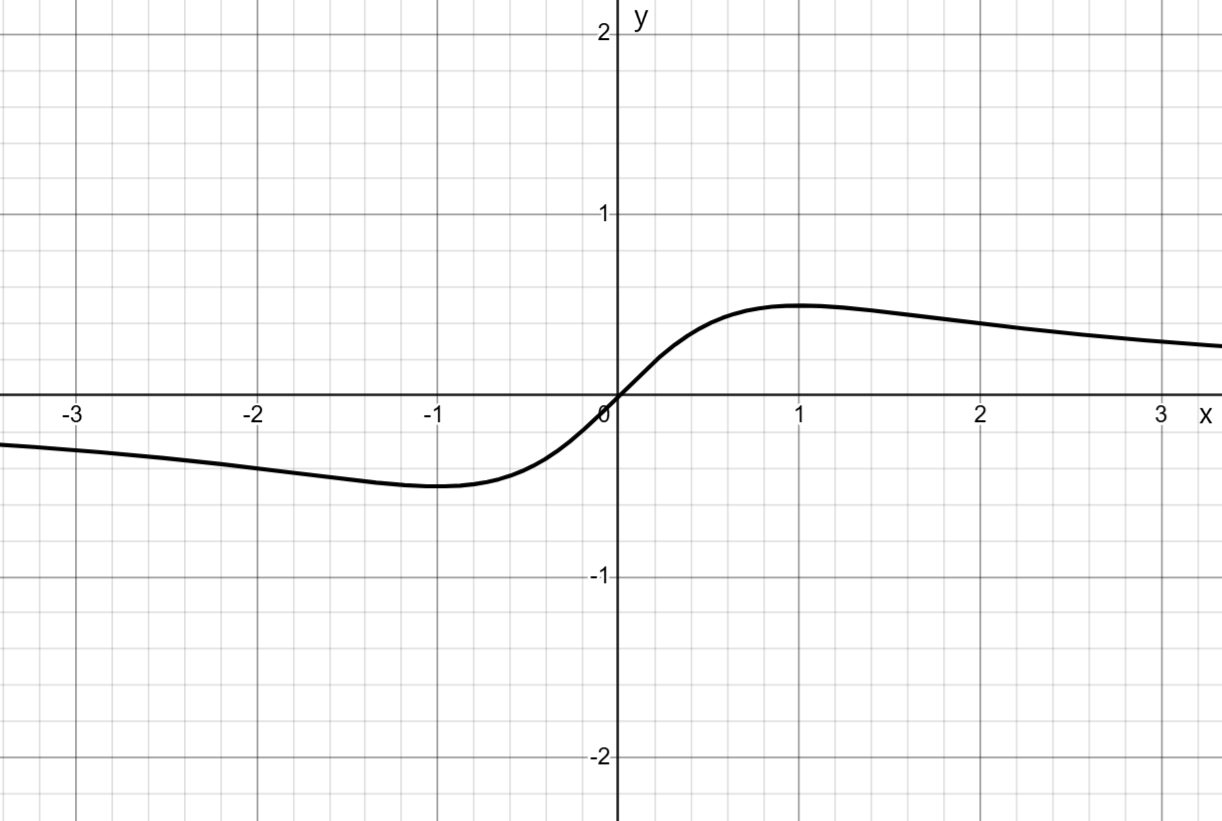
\includegraphics[width=0.8\linewidth]{img/18_graf_po_vysetreni.png}
        \caption{Graf vyšetření funkce} 
        \label{fig:enter-label}
    \end{figure}

Z grafu můžeme vyčíst, že $H(f)$ se pohybuje mezi minimem a maximem, tudíž $H(f) \in \langle -\frac{1}{2}; \frac{1}{2} \rangle$


